\chapter{Case Study II: Aluminium}%


%___________________________________________________________________________

\section*{\phantomsection%
  1. Metals and life%
  \addcontentsline{toc}{section}{1. Metals and life}%
  \label{metals-and-life}%
}

As it was advanced in the previous chapter, metals play an important role in several biological processes. They are central to a lot of essential biological reactions, but they can also be very toxic. As enunciated by Paracelsus, it's the dose that makes the poison. Life processes are very sensitive to concentration changes, especially when it comes to metal ions. As a result, if blood levels of a given metal experiments a sudden increase or decrease of concentration, it can lead to devastating consequences. For example, the most common case of anaemia is caused by iron deficiency: without iron, the cells cannot form enough functional haemoglobin to bind oxygen and support their metabolism.

Besides their metabolic implications, anomalies in the homeostasis of some metals have been reported to participate in some neurodegenerative disorders, such as Parkinson's (PD) or Alzheimer's (AD) disease. While AD is characterized by the accumulation of amyloid-beta plaques in the brain, its true etiology remains unknown. Aluminium has been in the spotlight since its brain accumulation was first described by \citet{Crapper1973}, amongst other metals \citep{Shcherbatykh2007, Gonzalez-Dominguez2014}. Although mainstream science seems to have abandoned the aluminium hypothesis due to some controversy in the previous studies \citep{Santibanez2007}, it still attracts some scientists \citep{Lidsky2014}.


%___________________________________________________________________________

\subsection*{\phantomsection%
  1.1. Aluminium as a biometal%
  \addcontentsline{toc}{subsection}{1.1. Aluminium as a biometal}%
  \label{aluminium-as-a-biometal}%
}

Aluminium(III) can coordinate to several different elements, but it particularly leans towards nitrogen and oxygen atoms in biological environments \citep{Kaim1994}, though oxygen is preferred due to its smaller size and larger negative charge. Thus, in a proteic environment, it will mostly bind to aspartic and glutamic acids, serine residues and the oxygens found in the backbone. The resulting coordinate complexes tend to feature coordination numbers of four, five and six \citep{GreenWood1997}, which usually means \emph{trigonal planar, tetrahedral and trigonal bipyramidal geometries} (\emph{\#! is this true?}), respectively.


%___________________________________________________________________________

\section*{\phantomsection%
  2. The challenge%
  \addcontentsline{toc}{section}{2. The challenge}%
  \label{the-challenge}%
}

Xabier López\footnote{Department of Science \& Technology of Polymer, Faculty of Chemistry, UPV/EHU} and coworkers are wondering if both observations can be compatible: does aluminium have something to do with amyloid-beta plaque accumulation? This case study tries to shed some light on the matter and discuss the possible results.


Dr. López supplied a set of GRID-optimized systems obtained from a PDB screening essay that looked for observed amyloid-beta structures, resulting in PDB entries 1AMB, 1AMC, 1AML, 1BA4, 1BA6, 1BJB, 1BJC, 1IYT, 1NMJ, 1Z0Q, 2LFM, 2M9R, and 2M9S. However, the GRID protocol used by López et al. only optimized the position of alpha-carbons while looking for energy minima, thus ignoring rotameric alterations and their chemosteric effects. Given the input library, we were asked to find the nearby oxygen-containing residues and optimize their rotameric configuration so they can allocate the aluminium in a feasible coordination geometry. Backbone oxygens were also allowed to participate in the complex, but their position should not be changed in order not to disrupt the tertiary structure of the protein.


%___________________________________________________________________________

\section*{\phantomsection%
  3. Current techniques in bioinformatics%
  \addcontentsline{toc}{section}{3. Current techniques in bioinformatics}%
  \label{current-techniques-in-bioinformatics}%
}

This case study can be regarded as a docking problem where the ligand is a single atom of aluminium. However, existent docking solutions rarely accept metals in the input, let alone being the naked ligand. Furthermore, rotameric optimization is usually directed towards hydrogen bond forming, Van der Waals contacts, and avoiding clashes, not towards the discovery of suitable coordination geometries. GOLD does implement this feature but is not optimized to handle them as part of the ligand \citep{Ortega-Carrasco2014}, and so does FlexX \citep{Seebeck2008}, but it does not support naked metal ions as ligands. Since GAUDI can be easily extended to adopt new objectives and features, we thought of creating an alternative launcher script that would meet the requirements of this essay.


%___________________________________________________________________________

\section*{\phantomsection%
  4. Our strategy%
  \addcontentsline{toc}{section}{4. Our strategy}%
  \label{our-strategy}%
}

GAUDI can treat any UCSF Chimera compatible input file as a ligand, so using a single aluminium atom as a ligand works out of the box. However, the provided dataset already included a tentative position for the aluminium, making that step unnecessary. Instead, the new script only had to detect existent aluminium atoms and register them as ligands. If more than one were found, only the one with the lowest serial number would be taken into account.

Once found, the initial set-up was performed. The aluminium was allowed to move to a random point within 2.5A of the starting position, and then search space field was created within 7.0A of the new position. If one or more oxygen atoms were found in the search sphere, their correspondent residues were registered in the rotamers optimization list. It mostly comprised aspartic and glutamic acids, and some serines too.

Detecting feasible coordination geometries can be an attractive feature and definitely will be implemented in the future, but for this essay it was not necessary. After choosing a new set of rotamers from the Dunbrack's library, the distances of the three nearest oxygen atoms were calculated, as well as the dihedral angle that their two immediate neighbours, themselves, and the aluminium ion formed. GAUDI was then set up to minimize both the distances to 2.2A with a minimum distance threshold of 1.8A, and the absolute sine of each of the dihedrals, seeking to obtain information about the planarity requirements of the coordinate residue, be it mono or bidentate. In order to avoid infeasible steric conformations, the clashes were calculated and minimized too. Least but not last, an additional scoring was added that accounted for the number of oxygen-containing residues found within 2.0A from the aluminium atom, which would give an approximate idea of the coordination number.

Since each of the 13 PDB entries contained several different poses, which in total accounted for 157 possible solutions, a helper script was designed to run all of them in batch. It simply consisted of a Python subprocess handler to launch sequential instances of UCSF Chimera. Each of the essays started with a population of 300 individuals and ran for 15 generations, with mu, lambda, and crossover probability set to 0.5, and mutation rate set to 0.2.


%___________________________________________________________________________

\section*{\phantomsection%
  5. Discussion of results%
  \addcontentsline{toc}{section}{5. Discussion of results}%
  \label{discussion-of-results}%
}

The generated Pareto front of solutions comprised more than 19,000 possible candidates, so an obvious filtering was needed. These were the applied restrictions.
%
\begin{quote}
%
\begin{itemize}

\item Clashes < 10 nm³

\item At least two oxygen atoms within 2.0A from the aluminium

\end{itemize}

\end{quote}

This configuration left us with 11 solutions. Of these 11, a total of five poses were chosen and proposed to Xabier. These were based on PDB entries 1AMC, 1AML, 1BJB, 1BJC, and 1Z0Q, whose details can be read in table Z. As it can be seen, the poses tend to feature three or four proximal oxygen atoms that would suggest an octahedral geometry. These atoms usually come from the carboxylic group of aspartic and glutamic acids, though some oxygen atoms from the atom can be also pointed out.

\begin{table}[h]
\centering
\caption{Details of the scoring of each proposed solutions. \emph{Nearby oxygens} refers to the number of oxygen atoms within 2.2A of the aluminium ion. \emph{Average distance} is calculated from the distance of the three nearest oxygens to the aluminium ion. \emph{Average planarity} is the mean of the absolute sines of the dihedrals formed with aluminium, oxygen, and the next two non-terminal atoms in the peptidic chain. A planarity of zero means that the chains are aligned, while a planarity of one means they are orthogonal. More details are given in Appendix A.}
\label{my-label}
\resizebox{\textwidth}{!}{%
\begin{tabular}{@{}lllll@{}}
\toprule
PDB code & Nearby oxygens & Clashes (nm³) & Average distance (nm) & Average planarity \\ \midrule
1AMC & 2 & 7.8922 & 2.6789 & 0.6433 \\
1AML & 2 & 6.1656 & 2.3198 & 0.9189 \\
1BJB & 2 & 7.6941 & 2.2176 & 0.5629 \\
1BJC & 2 & 8.1273 & 2.3761 & 0.8315 \\
1Z0Q & 2 & 9.665 & 2.3291 & 0.7289 \\ \bottomrule
\end{tabular}
}
\end{table}

\begin{figure}
\noindent\makebox[\textwidth][c]{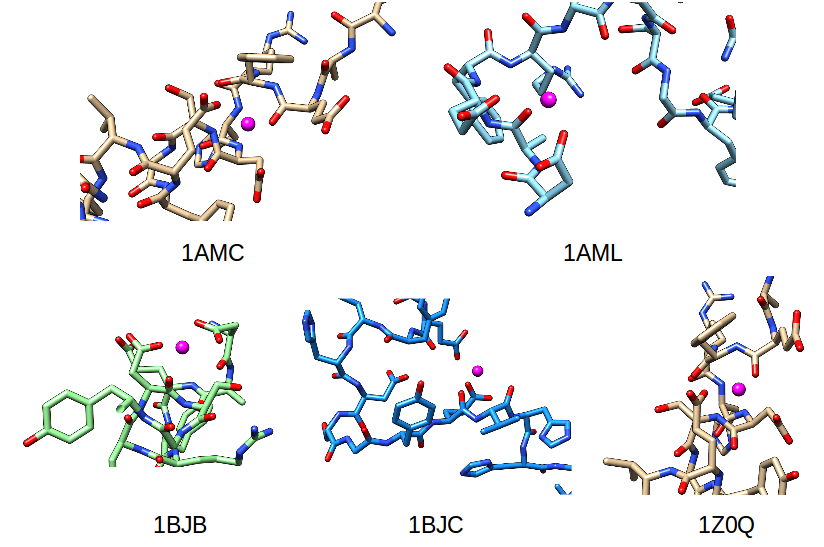
\includegraphics[width=\textwidth]{fig/results-aluminium.png}}
\caption{Selected solutions from the Pareto front proposed by the GAUDI essay. Aluminium ions are depicted in bright magenta.}
\end{figure}


\#! Conclusions!


